\documentclass[11pt]{article}

\usepackage[table]{xcolor}

\usepackage[
  letterpaper,
  left=0.65in,
  right=0.65in,
  top=0.35in,
  bottom=0.35in
]{geometry}

\usepackage{fontawesome5}
\usepackage[most]{tcolorbox}
\usepackage{graphicx}
\usepackage{parskip}
\usepackage{enumitem}
\usepackage{array}
\usepackage{tabularx}
\usepackage{multicol}
\usepackage{xcolor}
\usepackage{titlesec}
\usepackage{fancyhdr}
\usepackage{hyperref}
\usepackage{changepage}
\usepackage{float}
\usepackage{placeins}

\hypersetup{colorlinks=false,pdfborder={0 0 0}}

\usepackage{iftex}
\ifPDFTeX
  \usepackage[sfdefault]{carlito}
\else
  \usepackage{fontspec}
  \setmainfont{Georgia}
\fi

% Look for graphics in /images first, then in the project root.
\graphicspath{{images/}{./}}

\definecolor{DeepBlue}{RGB}{0,40,90}
\definecolor{CoursePurple}{RGB}{104,75,160}
\definecolor{CoursePurpleLight}{RGB}{245,242,252}

\setcounter{secnumdepth}{0}
\setlength{\parindent}{0pt}

\setlist[itemize]{leftmargin=1.4em,itemsep=0.2em,topsep=0.25em}
\setlist[enumerate]{leftmargin=1.6em,itemsep=0.2em,topsep=0.25em}

\titleformat{\section}{\Large\bfseries\color{DeepBlue}}{}{0em}{}
\titleformat{\subsection}{\normalsize\bfseries\color{DeepBlue}}{}{0em}{}

\titlespacing*{\section}{0pt}{1.1em}{0.35em}
\titlespacing*{\subsection}{0pt}{0.8em}{0.25em}

% Fine adjustment for tight syllabus sections.
\newcommand{\syllabusspacer}{0.1em}

\usepackage{changepage}

\newenvironment{subsectionbody}
{\begin{adjustwidth}{0.18in}{0pt}}
{\end{adjustwidth}}
\tcbset{
  syllabuscallout/.style={
    enhanced,
    colback=blue!2,
    colframe=DeepBlue,
    boxrule=0.8pt,
    arc=3pt,
    left=10pt,
    right=10pt,
    top=8pt,
    bottom=8pt
  }
}

\tcbset{
  coursetip/.style={
    enhanced,
    colback=CoursePurpleLight,
    colframe=CoursePurple,
    boxrule=0.8pt,
    arc=3pt,
    left=10pt,
    right=10pt,
    top=6pt,
    bottom=6pt
  }
}

\tcbset{
  contactcard/.style={
    enhanced,
    colback=white,
    colframe=DeepBlue,
    boxrule=0.8pt,
    arc=3pt,
    left=10pt,
    right=10pt,
    top=8pt,
    bottom=8pt,
    valign=top,
    before skip=0pt,
    after skip=0pt
  }
}

\newcommand{\contactcard}[6]{%
\begin{tcolorbox}[contactcard]
{\normalsize\bfseries\color{DeepBlue} #1}

\vspace{0.45em}

{\small
{\footnotesize\faMapMarker*} \hspace{0.5em} #2\par

\if\relax\detokenize{#3}\relax
\else
\vspace{0.25em}
{\footnotesize\faMapMarker*} \hspace{0.5em} #3\par
\fi

\vspace{0.35em}

{\footnotesize\faClock} \hspace{0.5em} #4\par

\vspace{0.35em}

{\footnotesize\faPhone} \hspace{0.5em} #5\par

\vspace{0.35em}

{\footnotesize\faEnvelope} \hspace{0.5em} \texttt{#6}
}
\end{tcolorbox}
}

% ========== Branding ==========
\newcommand{\institutionlogo}{SCC logo.jpg}

% ========== Header/Footer ==========
\pagestyle{fancy}
\fancyhf{}
\renewcommand{\headrulewidth}{0pt}






\begin{document}

% =====================================================
% COURSE HEADER WITH LOGO + TITLE BLOCK
% =====================================================

\vspace*{-0.15in}

\renewcommand{\arraystretch}{1}

\begin{tabularx}{\textwidth}{@{}m{2.95in}@{\hspace{0.45in}}>{\raggedleft\arraybackslash}X@{}}

\includegraphics[width=3in]{\institutionlogo}
&
\begin{minipage}[c]{\linewidth}
\raggedleft

{\Large\bfseries BIO 137 Human Anatomy \& Physiology I\par}

\vspace{0.4em}

{\normalsize
Summer 2026 \textbar{} 4 Credit Hours \textbar{} Online\par
Section E0Z9 \textbar{} Class 2787 \textbar{} SMC 4262\par
June 15 - August 7
}

\end{minipage}

\end{tabularx}

\vspace{0.55em}

{\color{DeepBlue}\rule{\textwidth}{0.8pt}}

\vspace{0.75em}

\section*{Course Contacts}


\begin{tabularx}{\textwidth}{@{}X@{\hspace{0.6cm}}X@{}}

\contactcard
{Instructor: Justin N. Howard}
{Somerset North Campus · Stoner Bldg · Rm 216}
{}
{Online: Blackboard for course issues; Email for urgent issues; message anytime; MS Teams, phone, or in-person meetings are welcome and encouraged.}
{606-451-6993}
{justin.howard@kctcs.edu}
&
\contactcard
{Associate Dean: April Kilgore, Ph.D.}
{Somerset North Campus · Stoner Bldg · Rm 210}
{Laurel North Campus · Bldg 2 · Rm 107}
{M--F 9:30 am--3:30 pm; appointments available as needed.}
{(606) 878-4755}
{april.kilgore@kctcs.edu}

\\[0.55cm]

\contactcard
{Administrative Assistant: Tammy Woodall}
{Somerset North Campus · Stoner Bldg · Rm 222}
{}
{Available during regular office hours for department and course-related assistance.}
{606-451-6704}
{tammy.woodall@kctcs.edu}
&
\contactcard
{Dean: John Burlew}
{Somerset Campus North · Stoner Bldg · Rm 210}
{}
{M--F 8:00 am--4:30 pm; appointments available as needed.}
{606-451-6748}
{jon.burlew@kctcs.edu}

\end{tabularx}

\vspace{0.5em}

\section*{Catalog Course Description}

BIO 137 Human Anatomy and Physiology I is an introduction to human anatomy and physiology. This course is the study of the interrelationship and structure and function of each body system in two semesters. The first semester will include basic chemistry, cell structure, cell physiology, metabolism, tissues, and integumentary, skeletal, muscular, and nervous systems.

The laboratory portion of BIO 137 is designed as a hands-on experience that corresponds to the lecture portion of the course. Anatomical models, computer programs, charts, slides of microscopic tissue sections, physiological experiments and preserved specimens for dissection will be used to reemphasize principles and structures discussed in lecture.


\newpage



\section*{Required Course Materials}

All course materials for this course are delivered through Blackboard, McGraw Hill, and Connect\textsuperscript{\textregistered}. These systems work together throughout the semester and are illustrated below.





\textbf{Blackboard} serves as the primary course portal. You should begin all course activities in Blackboard, where you will access announcements, course information, assignment links, grades, and instructor communications.

\textbf{McGraw Hill} is the publisher of your course textbook and provides the digital learning resources used throughout the semester.

\textbf{Connect\textsuperscript{\textregistered}} is McGraw Hill’s online learning platform. In this course, Connect may be used for SmartBook assignments, chapter activities, quizzes, exams, and access to the electronic textbook.



\begin{figure}[H]
    \centering
    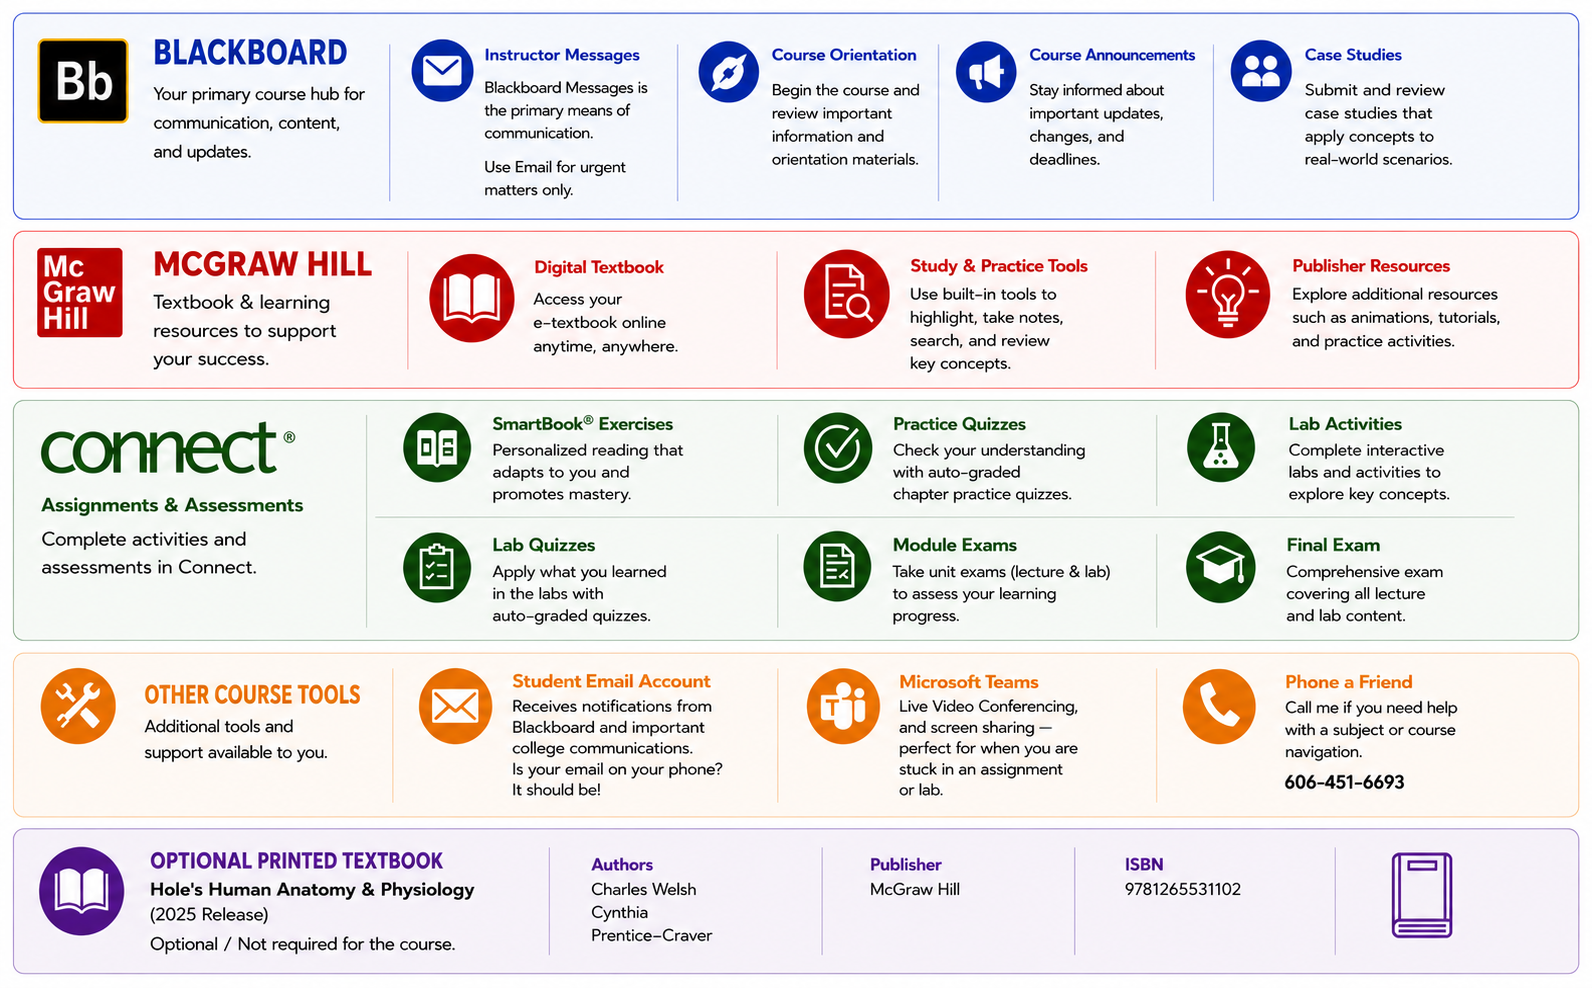
\includegraphics[width=1.01\textwidth]{course-materials-flow (2).png}
\end{figure}

Your required electronic textbook and Connect\textsuperscript{\textregistered} access are provided through the KCTCS Course Charge Model and are included as part of your course materials.

\newpage

\section*{Course Outline}

You should expect to spend approximately 8--20 hours per week reading your textbook, studying, and completing assignments for this class. Because this is an accelerated 8-week online course, students should plan to work consistently throughout the week and check Blackboard and KCTCS email daily. Details about the assignments are provided below.

\section*{Description of Assignments}

\begin{tcolorbox}[
  enhanced,
  colback=blue!2,
  colframe=DeepBlue,
  boxrule=0.8pt,
  arc=3pt,
  left=10pt,
  right=10pt,
  top=8pt,
  bottom=8pt
]
{\bfseries\color{DeepBlue} Course Point Summary}

\vspace{0.4em}

\renewcommand{\arraystretch}{1.22}
\begin{tabularx}{\linewidth}{@{}X c c r@{}}
\textbf{Assignment Category} &
\textbf{Number of Assignments} &
\textbf{Point Value} &
\textbf{Category Point Total} \\
\hline
Start Here Assignments & 5 & Varies & 37 \\
Interactive SmartBook Exercises & 12 & 20 & 240 \\
Chapter Practice Quizzes & 12 & 20 & 240 \\
Case Studies & 4 & 20 & 80 \\
Lab Exercises & 12 & 12 & 144 \\
Lab Quizzes & 12 & 12 & 144 \\
Module Exams & 4 & 100 & 400 \\
Final Review Quizzes & 8 & Varies & 20 \\
Final Exam & 1 & 100 & 100 \\
\hline
\textbf{Total} & \textbf{66} & -- & \textbf{1405} \\
\end{tabularx}
\end{tcolorbox}

\section{Start Here Assignments}

\textbf{These assignments are used as evidence of attendance during the first week of class. Because this is an accelerated 8-week online course, students must complete the first Start Here assignments early in the semester to remain enrolled and to gain access to the rest of the course.} \textit{Students who do not complete the required first-week attendance assignments may be dropped from the course without notification as per home campus procedures.}

The \textbf{Syllabus Quiz}, \textbf{Online Learning Survey}, and \textbf{Discussion Board} must be completed by \textbf{Thursday, June 18, 2026, at 11:59 p.m. eastern time}. Additional Start Here assignments, including \textbf{Succeeding in the Online Classroom} and \textbf{Fundamentals of Student Success}, must be completed by \textbf{Saturday, June 20, 2026, at 11:59 p.m. eastern time}.



\subsection{Below you will find a brief description of each of the Start Here Assignments:}

\textbf{Online Learning Survey (5 pts)} -- This is a true/false survey to indicate your readiness to succeed in an online course. The more true answers you have, the more likely you are to succeed in an online class. If you select false for one or more questions, you should carefully consider the time, technology, and study habits required to succeed in an online course.

\textbf{Syllabus Quiz (5 pts)} -- This important quiz ensures that you are familiar with important class policies before beginning your work. It must be repeated until you earn 5 out of 5 points. You will not have access to course assignments until you earn a perfect score on this quiz.

\textbf{Discussion Board: Let's get to know each other! (5 pts)} -- This discussion board assignment allows us to get to know each other. Please use this as an opportunity to connect with other students if you wish to establish an online or in-person study group.

\textbf{Succeeding in the Online Classroom (12 pts)} -- This assignment is designed to help you get familiar with the online learning environment. You will be introduced to the idea of a Learning Management System. That is the program you use to access your class. For us, that program is Blackboard.

\textbf{Fundamentals of Student Success (10 pts)} -- This assignment is designed to help you make the most of your studies of human anatomy and physiology by implementing effective study skills, time management strategies, organizational skills, understanding and maximizing your learning style, and how to effectively engage with the material you are studying, your classmates, and instructor.

\clearpage

\section*{Weekly Assignments}

Three to five assignments are due every 2--3 days every single week of the semester, \textbf{even during exam weeks, holidays, and breaks.} It is recommended that you complete them in the following order:

\begin{itemize}
  \item Read each chapter (0 points)
  \item Interactive SmartBook Exercises
  \item Chapter Practice Quizzes
  \item Case Studies
  \item Lab Exercises
  \item Lab Quizzes
\end{itemize}

\subsection*{Interactive SmartBook Exercises: Read and Answer Questions (20 points each, 240 points total)}

This course covers a total of 12 chapters. Each chapter begins with an assignment known as an Interactive SmartBook Exercise to help guide you through the important concepts in each chapter. There are a total of 12 SmartBook exercises worth 20 points each for a total of 240 points. These exercises have no time limit and may be repeated as many times as you wish before the due date to earn a perfect score for each assignment. Each exercise is designed to take the average student approximately 1 hour to complete, so schedule your time accordingly. Waiting until the last minute will reduce the number of attempts you can make at each exercise.

\begin{tcolorbox}[coursetip]
{\bfseries Important Note About SmartBook}

SmartBook assignments begin with questions, but you are not expected to answer everything from memory. As you work, you may switch back and forth between answering questions and reading the electronic textbook. The program is interactive and may recommend specific readings or topics for review based on your responses. Students often find that moving between the questions and the textbook helps them learn the material more efficiently.
\end{tcolorbox}

\subsection*{Chapter Practice Quizzes (20 points each, 240 points total)}

After reading and completing the SmartBook exercise for each chapter, you must complete a quiz over the same content covered in the SmartBook exercise. These quizzes will test your ability to remember and apply what you covered in SmartBook exercises. You may use your textbook and notes, but a 30-minute time limit will be imposed. You may repeat the quiz, beginning with an entirely new set of questions, up to 3 times. Your best score will be used for grading purposes. You will complete a total of 12 Practice Quizzes, 1 per chapter, worth 20 points each for a total of 240 points.

\subsection*{Case Studies (20 points each, 80 points total)}

Four Case Studies are assigned, one at the end of each module. They are designed to help you apply concepts from each chapter in a real-life situation. Responses are submitted in Blackboard. Each of the four case study assignments is worth 20 points for a total of 80 points.

\subsection*{Lab Exercises (12 points each, 144 points total)}

The laboratory portion of the course is presented in an entirely online format using Anatomy \& Physiology Revealed (APR), and Virtual Labs. Each of the 12 lab activities will involve one or both of those programs; some labs have two parts. The lab exercises may be completed an unlimited number of times before the due date and only your highest score will be used for grading. After the due date you may revisit the labs for review only. Later attempts will not increase your grade. Importantly, these lab exercises also prepare you for the weekly lab quizzes. Questions on the lab quizzes are taken directly from these assignments. Each lab exercise is worth 12 points for a total of 144 points.

\subsection*{Lab Quizzes (12 points each, 144 points total)}

Upon completing each lab activity, students may proceed to a lab quiz designed to assess understanding of key concepts from the laboratory activity. Lab quizzes are limited to 30 minutes. These quizzes may be repeated up to 3 times, only the highest score will be used for grading. A total of 12 lab quizzes are assigned worth 12 points each for a total of 144 points.

\section*{Exams}

\subsection*{Module Exams (400 points total; 240 from lecture, 160 from lab)}

Module exams will be assigned at the end of each 3-chapter module. Module assignments are due before the exam window opens. Exams will open according to the schedule posted in Blackboard and will remain available during the posted exam window. Exams can be taken any time during the exam window, but they cannot be repeated for higher scores within that time.

Each module contains a separate exam for lecture and lab. The lecture portion of the exam will be taken from material covered in each chapter of the text that you have practiced through SmartBook Exercises, Chapter Practice Quizzes, and case studies. The lecture portion of each module exam will contain 30 questions worth 2 points each for a total of 60 points. You will have 60 minutes to complete the lecture portion of each module exam.

The laboratory portion of the exam will cover concepts, skills, and memorization information contained in each laboratory exercise. The laboratory portion of each module exam will contain 20 questions worth 2 points each for a total of 40 points. You will have 40 minutes to complete the laboratory portion of each module exam.

The combined value of each lecture and laboratory module exam is 100 points. There are four module exams, so a total of 400 possible points for exams throughout the semester.

\subsection*{Final Review Quizzes (20 points total)}

The week before your final exam opens, you will have the opportunity to review concepts from throughout the course by completing final review quizzes. These review quizzes are divided by module and by lecture/lab content. Together, they are worth a total of 20 points. Per the discretion of your instructor, you may also have bonus assignments to help you review for the final.

\subsection*{Final Exam (100 points total; 60 from lecture, 40 from lab)}

The final exam will be a comprehensive exam covering all 12 lecture chapters and all 12 lab activities from the course. The lecture and laboratory portions will be administered separately. Both portions will be available during the final exam window posted in Blackboard. Your answers must be submitted before the deadline to earn credit for the final exam.

The final exam lecture portion will consist of 60 questions from lecture material worth 1 point each. You will have 120 minutes to complete this portion of the exam. The final exam laboratory portion will contain 40 questions from laboratory material worth 1 point each. You will have 80 minutes to complete the laboratory portion of the exam.

\newpage 

\section*{Grading Criteria}

A standard grading scale with rounding at the 0.5\% mark will be used: A = 89.5\% or above; B = 79.5--89.4\%; C = 69.5--79.4\%; D = 59.5--69.4\%; E = below 59.5\%.

A total of 1405 points, not including bonus assignments, can be earned by the end of the semester after completing all assignments. The total points earned at the end of the semester is divided by 1405 to determine your final course grade.

\begin{tcolorbox}[
  enhanced,
  colback=blue!2,
  colframe=DeepBlue,
  boxrule=0.8pt,
  arc=3pt,
  left=10pt,
  right=10pt,
  top=8pt,
  bottom=8pt
]
{\bfseries\color{DeepBlue} Grade Scale}

\vspace{0.25em}

\textbf{A} --- To earn an A, students must have 1258 or more points. This is equivalent to 89.5\% or above.

\vspace{0.2em}

\textbf{B} --- To earn a B, students must have 1117 to 1257 points. This is equivalent to 79.5 to 89.4\%.

\vspace{0.2em}

\textbf{C} --- To earn a C, students must have 977 to 1116 points. This is equivalent to 69.5 to 79.4\%.

\vspace{0.2em}

\textbf{D} --- To earn a D, students must have 836 to 976 points. This is equivalent to 59.5 to 69.4\%.

\vspace{0.2em}

\textbf{E} --- To earn an E, students must earn 835 or fewer points. This is equivalent to below 59.5\%.
\end{tcolorbox}

\subsection*{Determining Your Grade Throughout the Semester}

After each major course deadline, you should evaluate your progress by dividing the total points you've earned on that date by the total number of points possible at that point in the course. This will give you a percentage score and allow you to determine your standing in the course. Please do NOT use the percentage provided in Blackboard alone as it may not always accurately reflect your grade. Please use the point information provided in the master course schedule and the assignment list in Blackboard to determine your grade at any time during the semester. \textbf{Email or call me at any time if you have questions about your grade.}

\section*{Attendance Statement}

Your attendance is determined by completion of assigned material. You are expected to access course materials online in Blackboard and check your KCTCS email account daily. You are responsible for all posted announcements, assignments, quizzes, and exams.

Because this is an accelerated 8-week online course, attendance begins with completion of the required Start Here assignments during the first week of class. Students who do not complete the required first-week attendance assignments may be dropped from the course without notification as per home campus procedures.

Additional assignments are due, on average, every 2--3 days at 11:59 p.m. eastern time. Case Study assignments are due at the end of each 3-chapter module. Each of the four Module Lecture and Lab Exams will be completed at the end of the corresponding 3-chapter module. See the course schedule in Blackboard for all official due dates.

\section*{Late Assignments and Make-Up Policy}

Assignments, lab activities, SmartBook assignments, and quizzes are due on the dates listed in the course schedule. Most assignments include an automatic two-day extension period beyond the original due date. Students may continue working during this extension period without contacting me.

After the late submission deadline has passed, the assignment will close and no additional submissions will be accepted. Because all students receive the same automatic extension opportunity, individual requests to reopen assignments are generally not granted.

Students are encouraged to complete assignments by the original due date whenever possible. The two-day extension period is intended to provide flexibility for unexpected events, scheduling conflicts, work obligations, and minor technical difficulties while helping students remain on pace with the course.

Module exams and final exams should be completed by the scheduled deadline. Students who miss a module exam may be eligible for one make-up exam opportunity near the end of the semester. Information regarding the make-up exam process will be provided during the final weeks of the course.

If a significant emergency or extended absence affects your ability to complete coursework, please contact me as soon as possible to discuss available options.

\newpage

\section*{Withdrawal Policy}

A student may officially withdraw from any class up to and including the date of midterm with a W grade. After the date of midterm and through the last class of the semester or session, any student may officially request to withdraw from a course and receive a W, which may be given at the discretion of the instructor.

Withdrawal requests will only be approved if the student has continued working in class and at least 80\% of the coursework to that date is completed with a grade more than 0. An instructor shall not assign a student a W for a class unless the student has officially withdrawn from that class in a manner prescribed by the college. The grade of W may be assigned by the College Appeals Board in classes involving a violation of student academic rights or for academic offenses. Please refer to the Student Records Office for more information.


\section*{Academic Integrity}

Students must complete their own work. Academic dishonesty will not be tolerated. A first offense will result in a failing grade on the assignment. A second offense will result in a failing grade for the course.

Please refer to the SCC Student Code of Conduct for more information.

\section*{Accessibility Services for Students with Disabilities}

Somerset Community College strives to make learning experiences accessible to all participants and is committed to providing reasonable accommodation for all persons with disabilities. If you are seeking accommodations for this course under the Americans with Disabilities Act (ADA), you are required to contact the Accessibility/Disabilities Services Office.

To request accommodations, complete the Student Request for Services form. Please do not request accommodation directly from your instructor without a letter of accommodation from the Accessibility/Disability Services Office.

If you are a student from a KCTCS college other than Somerset Community College, contact your Home College for establishing disability accommodations. You can find your Home College's Accessibility/Disability Services Office contact information on the KCTCS Disability Services site. Your Home College will communicate with your instructors and Accessibility/Disability Services Office to provide you with reasonable and appropriate accommodation. Your accommodations will begin after the instructor has received confirmation of your accommodation from the Accessibility/Disability Services Office. Accommodation cannot be applied to your course retroactively.

\begin{tcolorbox}[coursetip]
{\bfseries Accessibility Services Contact Information}

\vspace{0.3em}

\renewcommand{\arraystretch}{1.1}
\begin{tabularx}{\linewidth}{@{}>{\bfseries}l X@{}}
Coordinator: & \textbf{Amanda Vanhook} \\
Email: & amanda.vanhook@kctcs.edu \\
Office Email: & SCC-Accessibility@kctcs.edu \\
Phone: & 606-451-6706 \\
Appointments: & In-person, virtual, and phone appointments available \\
Somerset Office: & Hal Rogers Student Commons Building, Office 116 \\
Laurel Office: & Building 3, Office 103B \\
\end{tabularx}

\end{tcolorbox}

\section*{Procedures Relating to Discrimination, Harassment, and Sexual Misconduct}

Students may direct complaints of discrimination or harassment to Dean of Student Affairs Tracy Casada at \\
\textbf{tracy.casada@kctcs.edu or 606-451-6631} for resolution pursuant to the Code of Student Conduct. Sexual misconduct matters should be directed to the Title IX Coordinator Tracy Casada to be handled in accordance with the Sexual Misconduct Procedure. Any responsible employee who receives information related to sexual misconduct is required to report it to the Title IX Coordinator. Please refer to the KCTCS Title IX procedures for more information.

\clearpage

\section*{Student Academic and Technical Support}

Somerset Community College offers support to all its students, whether enrolled in classes on campus or online. Your instructor is your primary resource, but the Learning Commons branches are available for assistance with research, tutoring, and computer services. Tutoring appointments can be made online but are not necessary. Walk-ins are welcome. Students can also access contact information and hours of operation for all the branches of the Learning Commons. For more information, call 606-451-6710.

\begin{tcolorbox}[coursetip]
{\bfseries Technical Support}

Blackboard technical support is available by telephone at 855-664-6722, option 4.
\end{tcolorbox}



\section*{Starfish}

SCC is dedicated to your academic success. Starfish is a program available to all students to enhance communication among students, instructors, and advisors. To access Starfish, just log in to Blackboard and click Starfish link. Ask your instructor or advisor for details. Check out SCC's website for more details and helpful instructions.

\section*{SNAP}

Safety Notification Alert Process (SNAP) is the official notification system for the Kentucky Community and Technical College System (KCTCS). SNAP alerts users to on-campus emergencies, including closures for inclement weather, for all 16 KCTCS colleges and the System office. With SNAP you can:

\begin{itemize}
\item Find out if classes are cancelled or delayed due to weather, power outages, or other unexpected events impacting campus.
\item Get severe weather notifications so you can take shelter when a storm hits.
\item Receive emergency messages when something or someone could be a threat to your personal safety.
\end{itemize}

Visit the KCTCS SNAP site to sign up and/or update your mobile and email information.

\section*{KCTCS/SCC Tobacco Free Policy}

``Tobacco use, including chewing (oral), smoking, and electronic cigarettes are not permitted on the properties of Somerset Community College campuses and centers, including buildings, sidewalks, and parking lots. KCTCS Tobacco Free Policy, Administrative Policies, Section 3.3.14.'' Please refer to the KCTCS Administrative Policies for additional information.

\section*{Additional Information}

The College must remain flexible to meet challenges that may include epidemics, pandemics, natural disasters, human-influenced disasters, and any and all threats to the College campus, students, employees, and surrounding communities. To ensure the safety and well-being of our constituencies, the College maintains the right to move classes temporarily or permanently to online, remote platforms; to a hybrid section that includes some face-to-face learning and some remote learning; or to a different campus, location, building, or time.

Additionally, the College reserves the right to institute plans or practices in the physical classroom/lab/activity spaces and common areas to protect students and employees. The College will attempt to make these changes as minimally disruptive as possible, but the College reserves the sole right to alter the particular type, place, or time for their classes.



\end{document}
